\section{The experiment}
This work focuses on comparing the different misuse models to a reference
calculation in which a single large cascade is build and designed to directly
produce \gls{HEU} from natural uranium.
This works uses the Cyclus fuel cycle simulator to allow material exchange
between facilities. The enrichment cascade algorithm have been implemented in
the $mbmore$ package \cite{mbmore.2018}.
In each cases, 5060 centrifuges have been used and spread across up to 30
different gas centrifuge enrichment cascades. 


\subsection{The cascade configuration}

\subsubsection{Reference}

As mentioned, all the further calculations will be compared to the most
favorable configuration to produce \gls{HEU}, where all the available
centrifuges are used in a single large ideal symmetric cascade designed to
directly produce \gls{HEU} from natural uranium, with a tails assay close to
$0.3w\%$. The design characteristic of the reference cascade are summarized in
Table \ref{tab:cascade_config}.

\subsubsection{Default cascade}

The default cascade is the ideal symmetric cascade designed for normal civilian
enrichment operation, enriching natural uranium to about $3.5w\%$, with a tails
assay close to $0.3w\%$. This cascade will be layered and fed with uranium at
higher enrichment to evaluate the possibility to use them, with little or no
tuning, to produce \gls{HEU}. The characteristics of the default cascade are
summarized in Table \ref{tab:cascade_config}.

\begin{table}[htb]
\centering
  \caption{Summary of cascade design.}
\begin{tabular}{cccc}
\toprule

Cascade Design &       & Reference   & Default    \\
\midrule
Targeted  & Feed       & $0.71w\%$   & $0.71w\%$  \\
Assays    & Product    & $90w\%$     & $3.5w\%$   \\
          & Tails      & $0.3w\%$   & $0.3w\%$   \\
\midrule
Effective & Product    & $90.35w\%$  & $4.13w\%$  \\
Assays    & Tails      & $0.29w\%$   & $0.29w\%$  \\ 
\midrule
Stages    & Stripping  & 4          & 4          \\
Number    & Enriching  & 39         & 10         \\
\bottomrule
\end{tabular}
  \label{tab:cascade_config}
\end{table}


\subsection{Scenarios}
In the following, cascades can be connected in tandem, where each set of cascade
in parallel is called a ``level``, as illustrated in Figure
\ref{fig:cascade_level}.
The reseults from seven different simulations have been compared, to evaluate the effectiveness
of an enrichment cascade when used outside of its designed scope :
\begin{itemize}
\item one as the reference calculation, with a single cascade designed to
    directly produce \gls{HEU} from natural uranium,
\item three calculations (one per misuse model) where default cascade are
    chained to produce \gls{HEU}, without recycling the tails of each cascade
    sending their tails to the waste,
\item three calculations (one per misuse model) where default cascade are
    chained to produce \gls{HEU}, and the tails of each cascade are recycled, blending
    the tails of one level in the feed of the previous level of
    cascades (see Figure \ref{fig:cascade_level}).
\end{itemize}

\begin{figure}[ht] % replace 't' with 'b' to force it to be on the bottom
    \centering
    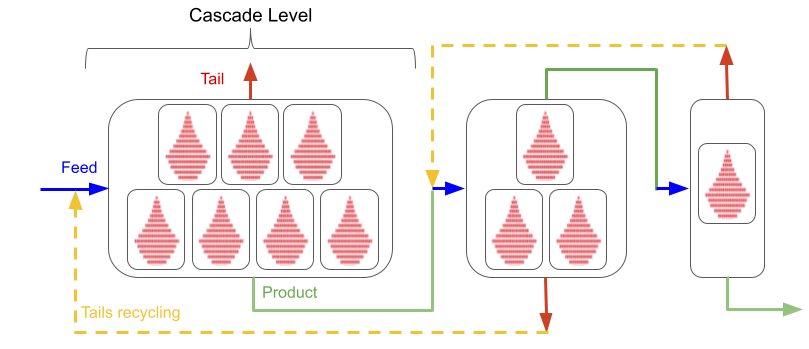
\includegraphics[width=\linewidth]{flow}
    \caption{Schematic representation of the chained cascades with three levels,
    with the feed, product and the tails flows, in blue, green and red,
    respectively. The dashed orange line represent the alternative tails flow when
    tails recycling is considered.}
    \label{fig:cascade_level}
\end{figure}


\subsection{Level population}
In order to assign the optimum number of cascades to each level, a ``level cut'' as
been computed as:
\begin{equation}
    \Omega_{j} = \frac{N_{j}-N''_{j}}{N'_{j}-N''_{j}},
\end{equation}
where, $j$ represents a level of cascade and $N_{j}$, $N'_{j}$ and $N''_{j}$
the feed, product and tails assay, respectively, of the cascades at this level.

A flow equation similar to \eqref{eq:flow} is then solved to obtain the optimum
number of cascade per level. When the tails are not recycled, the $(1-\theta)$
terms are removed from the flow equation.  The results of the level population
are summarized in Table \ref{tab:level}.

As it is not possible to assign a fraction of an enrichment cascade, cascade per
level are rounded up for each level but the first one. The remaining available
cascades are attributed to the first level.


%% \subsection{Timestep effect}
%% 
%% The different cascade levels required up to $2n+1$ timesteps
%% before it starts to enrich uranium, where $n$ corresponds to the level number.
%% This corresponds to the number of timesteps required for the material to
%% propagate from the natural uranium source to the $n$-th level, regardless of the
%% duration of the timestep (hour, day, month, etc.). This is also true for the
%% number of timesteps required to reach the equilibrium assays value in the tails
%% reprocessing cases.  As timestep can be artificially small or large, one will
%% only be considering equilibrium values of flow rates and assays in the following
%% analysis.
